\documentclass[../TheoreticalMechanics.tex]{subfiles}

\begin{document}

\graphicspath{{RigidBody/}}

\section{刚体运动} % (fold)
\label{sec:刚体运动}

\subsection{运动学} % (fold)
\label{sub:运动学}

\subsubsection{运动坐标} % (fold)
\label{ssub:运动坐标}

\begin{lemma}[刚体自由度]
    刚体运动最多有$6$个自由度.
\end{lemma}
\begin{lemma}[坐标变换]
    设有标架$\pare{\ve_1, \ve_2, \ve_3}$到$\pare{\ve'_1,\ve'_2,\ve'_3}$的变换, 记
    \[ \cos\theta_{ij} = \ve'_i \cdot \ve_j,\quad \vA = \pare{\cos\theta_{ij}}. \]
    \[ \begin{pmatrix}
        \ve'_1 & \ve'_2 & \ve'_3
    \end{pmatrix}^T = \vA \begin{pmatrix}
        \ve_1 & \ve_2 & \ve_3
    \end{pmatrix}^T,\quad \begin{pmatrix}
        x' & y' & z'
    \end{pmatrix}^T = \vA \begin{pmatrix}
        x & y & z
    \end{pmatrix}^T. \]
\end{lemma}
\begin{lemma}[坐标变换的自由度]
    正交标架的坐标变换矩阵$\vA$满足$\vA\vA^T=\vI$, 故$\vA$仅有$3$个自由度.
\end{lemma}
\begin{lemma}[坐标变换保持行列式]
    物理上可行的坐标变换$\vA$满足$\det\vA = 1$.
\end{lemma}
\begin{lemma}[坐标变换的相对性]
    坐标变换的矩阵可视为关联在新的基下的分量, 也可以视为关联在相同基下反变换后的分量.
\end{lemma}
\begin{lemma}[坐标变换下的矩阵]
    设$\vA$为基变换矩阵, 则线性算子$\vT$在新的基下有形式
    \[ \vT' = \vA \vT \vA^{-1}. \]
    如果$\vA=\pare{a_{ij}}$, $\vT = \pare{t_{kl}}$, 则
    \[ t'_{kl} = a_{ik}a_{jl}t_{kl}. \]
\end{lemma}
\begin{theorem}[Euler角相应的矩阵]
    \label{thm:Euler角相应的矩阵}
    如\cref{fig:Euler角的旋转次序}中的旋转相应的矩阵为
    \[ \begin{pmatrix}
        \cos\psi\cos\phi - \cos\theta\sin\phi\sin\psi & \cos\psi\sin\phi+\cos\theta\cos\phi\sin\psi & \sin\psi\sin\theta \\
        -\sin\psi\cos\phi-\cos\theta\sin\phi\cos\psi & -\sin\psi\sin\phi + \cos\theta\cos\phi\cos\psi & \cos\psi\sin\theta \\
        \sin\theta\sin\phi & -\sin\theta\cos\phi & \cos\theta
    \end{pmatrix}. \]
\end{theorem}
\begin{figure}[ht]
    \centering
    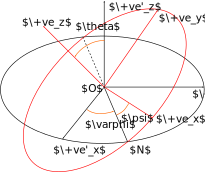
\includegraphics[width=.7\textwidth]{src/EulerAngles.eps}
    \caption{旋转次序为$\phi\rightarrow \theta\rightarrow\psi$}
    \label{fig:Euler角的旋转次序}
\end{figure}
\begin{remark}
    Euler角的顺序可能在不同文献中有所不同. 只要没有连续绕相同轴的两次旋转都是可行的. 另外的Tait-Bryan顺序为航向-俯仰-侧滚.
\end{remark}
\begin{ex}
    还可以通过Cayley-Klein参数化表示旋转.
\end{ex}
\begin{finale}
    \begin{theorem}[Euler定理]
        刚体在空间中的定点运动是绕某个点的转动. 将该点作为原点, 则刚体的定点运动可视为随体坐标系的旋转.
    \end{theorem}
\end{finale}
\begin{remark}
    还可以有更强的Chasles定理, 即刚体的一般运动总能分解为平移加旋转, 且有通过选取刚体随体坐标系的原点使旋转轴为平移轴.
\end{remark}
\begin{lemma}[旋转的向量表示]
    在坐标系绕$\vn$逆时针旋转$\Phi$后, 向量$\vr$变为
    \[ \vr' = \vr\cos\Phi + \vn\pare{\vn\cdot\vr}\pare{1-\cos\Phi} + \pare{\vr\times\vn}\sin\Phi. \]
\end{lemma}
\begin{lemma}[旋转角与Euler角的关系]
    绕某轴的旋转与相应的Euler角之间有关系
    \[ \cos\frac{\Phi}{2} = \cos\frac{\phi + \psi}{2}\cos\frac{\theta}{2}. \]
\end{lemma}
\begin{proof}
    由\cref{thm:Euler角相应的矩阵}与矩阵的迹的不变性可得.
\end{proof}
\begin{lemma}[无限小旋转的Euler矩阵]
    \label{lem:无限小旋转的Euler矩阵}
    在无限小旋转下, Euler矩阵变为
    \[ \vA = \begin{pmatrix}
        1 & \pare{\rd{\phi} + \rd{\psi}} & 0 \\
        -\pare{\rd{\phi} + \rd{\psi}} & 1 & \rd{\theta} \\
        0 & -\rd{\theta} & 1
    \end{pmatrix}\quad \Longleftrightarrow \quad \rd{\Omega} = \vi\,\rd{\theta} + \vk\pare{\rd{\phi} + \rd{\psi}}. \]
\end{lemma}
\begin{lemma}[一般旋转微元]
    设旋转矩阵为$\vA = \vI + \vepsilon$, 其中
    \[ \vepsilon = \begin{pmatrix}
        0 & \rd{\Omega_3} & -\rd{\Omega_2} \\
        -\rd{\Omega_3} & 0 & \rd{\Omega_1} \\
        \rd{\Omega_2} & -\rd{\Omega_1} & 0
    \end{pmatrix}, \]
    则$\rd{\vr} = \vA\vr - \vr = \vr\times\rd{\vOmega}$.
\end{lemma}
\begin{finale}
    \begin{corollary}[微小旋转可交换]
        两个连续的旋转微元可以交换.
    \end{corollary}
\end{finale}
\begin{remark}
    $\rd{\vOmega}$在保号旋转下按照向量的方式变化, 但在反号旋转下被镜面.
\end{remark}
\begin{corollary}[旋转微元的几何意义]
    $\rd{\vOmega} = \vn\,\rd{\Phi}$.
\end{corollary}
\begin{lemma}[向量旋转的表示]
    向量$\vr$绕$\vn$逆时针旋转$\Phi$后变为
    \[ \vr' = \vr\cos\Phi + \vn\pare{\vn\cdot\vr}\pare{1-\cos\Phi} + \pare{\vn\times\vr}\sin\Phi. \]
\end{lemma}
\begin{lemma}[向量的旋转微元表示]
    向量$\vr$绕$\vn$逆时针旋转$\rd{\Phi}$时满足
    \[ \eddon{\vr}{\rd{\Phi}} = \vN \vr. \]
    其中
    \[ \vepsilon = \begin{pmatrix}
        0 & -\rd{\Omega_3} & \rd{\Omega_2} \\
        \rd{\Omega_3} & 0 & -\rd{\Omega_1} \\
        -\rd{\Omega_2} & \rd{\Omega_1} & 0
    \end{pmatrix} = \begin{pmatrix}
        0 & -n_3 & n_2 \\
        n_3 & 0 & -n_1 \\
        -n_2 & n_1 & 0
    \end{pmatrix}\rd{\Phi} = \vN\,\rd{\Phi}. \]
\end{lemma}
\begin{lemma}[旋转生成元]
    \label{lem:旋转生成元}
    $\vepsilon = n_i\vM_i\,\rd{\Phi}$, 其中
    \[ \vM_1 = \begin{pmatrix}
        0 & 0 & 0 \\
        0 & 0 & -1 \\
        0 & 1 & 0
    \end{pmatrix},\quad \vM_2 = \begin{pmatrix}
        0 & 0 & 1 \\
        0 & 0 & 0 \\
        -1 & 0 & 0
    \end{pmatrix},\quad \vM_3 = \begin{pmatrix}
        0 & -1 & 0 \\
        1 & 0 & 0 \\
        0 & 0 & 0
    \end{pmatrix}, \]
    且成立$\brac{\vM_i,\vM_j} = \epsilon_{ijk}\vM_k$.
\end{lemma}

% subsubsection 运动坐标 (end)

\subsubsection{微分变换} % (fold)
\label{ssub:微分变换}

\begin{lemma}[刚体上向量的变化率]
    设有刚体上向量$\vG$, 则$\vG$的变化率可分为在随体坐标系内可观测到的变化与由刚体旋转导致的变化两部分, 即
    \[ \pare{\rd{\vG}}_{\mathrm{space}} = \pare{\rd{G}}_{\mathrm{body}} + \pare{\rd{\vG}}_{\mathrm{rot}}. \]
    并且成立
    \[ \pare{\rd{\vG}}_{\mathrm{rot}} = \rd{\vG}\times\vG. \]
\end{lemma}
\begin{finale}
    \begin{theorem}[随体导数]
        设有刚体上向量$\vG$且刚体的具有顺时角速度$\vomega$, 则
        \begin{equation}
            \label{eq:刚体随体导数}
            \pare{\eddon{\vG}{t}}_{\mathrm{space}} = \pare{\eddon{\vG}{t}}_{\mathrm{body}} + \vomega\times\vG.
        \end{equation}
    \end{theorem}
\end{finale}
\begin{theorem}[角速度在体坐标系下]
    \label{thm:角速度在体坐标系下}
    设刚体的旋转由Euler角给出, 则其角速度在体坐标系下为
    \begin{align*}
        \omega_{x'} &= \dot{\phi}\sin\theta\sin\psi + \dot{\theta}\cos\psi,\\
        \omega_{y'} &= \dot{\phi}\sin\theta\cos\psi - \dot{\theta}\sin\psi,\\
        \omega_{z'} &= \dot{\phi}\cos\theta + \dot{\psi}.
    \end{align*}
\end{theorem}
\begin{pitfall}
    \cref{lem:无限小旋转的Euler矩阵}和\cref{thm:角速度在体坐标系下}分别给出外坐标系和体坐标系下$\omega$的分量.
\end{pitfall}
\begin{ex}[Coriolis效应]
    地球上的运动物体成立
    \[ \vv_{\mathrm{space}} = \vv_{\mathrm{earth}} + \vomega\times\vr, \]
    \begin{align*}
        \pare{\eddon{\vv_{\mathrm{space}}}{t}}_{\mathrm{space}} &= \pare{\eddon{\vv_{\mathrm{space}}}{t}}_{\mathrm{earth}} + \vomega\times\vv_{\mathrm{space}}\\
        &= \vva_{\mathrm{earth}} + 2\pare{\vomega\times\vv_{\mathrm{earth}}} + \vomega\times\pare{\vomega\times\vr}.
    \end{align*}
    从而得到在地球上的运动方程
    \[ \vF_{\mathrm{eff}} = \vF - 2m\pare{\vomega\times\vv} - m\vomega\times\pare{\vomega\times\vr}. \]
\end{ex}

% subsubsection 微分变换 (end)

% subsection 运动学 (end)

\subsection{一般运动方程} % (fold)
\label{sub:一般运动方程}

\subsubsection{转动参量} % (fold)
\label{ssub:转动参量}

\begin{lemma}[变量分离]
    在质心系下, 有分解
    \[ T = \half Mv^2 + T'\pare{\phi,\theta,\psi}, \]
    其中$v$是质心速度. 势能亦可能类似的分解.
\end{lemma}
\begin{lemma}[角速度的坐标无关性]
    刚体的角速度与随体坐标的选择无关.
\end{lemma}
\begin{proof}
    设$\vR_1$和$\vR_2$为质点上二随体坐标的原点相对于外坐标系的位矢, $\vR = \vR_2-\vR_1$, 则由\eqref{eq:刚体随体导数},
    \[ \pare{\eddon{\vR_2}{t}}_{\mathrm{s}} = \pare{\eddon{\vR_1}{t}}_{\mathrm{s}} + \vomega_1\times\vR,\quad \pare{\eddon{\vR_1}{t}} = \pare{\eddon{\vR_2}{t}} - \vomega_2\times\vR. \]
    故$\pare{\vomega_1 - \vomega_2}\times\vR = 0$.
\end{proof}
\begin{finale}
    \begin{theorem}[转动惯量]
        对刚体定义转动惯量$\vI$满足
        \[ I_{jk} = \int_V \rho\pare{\vr}\pare{r^2 - \delta_{jk} x_j x_k}\,\rd{V}. \]
        则有
        \[ \vL = \int_V \rho\pare{\vr}\brac{\omega r^2 - \vr\pare{\vr\cdot\vomega}}\,\rd{V} = \vI \cdot\vomega. \]
    \end{theorem}
\end{finale}
\begin{lemma}[转动惯量作为对称矩阵]
    $I_{ij} = I_{ji}$.
\end{lemma}
\begin{lemma}[转动惯量的特征值]
    $\vI$有沿三个正交轴的特征值和特征向量满足
    \[ L_1 = I_1 \omega_1,\quad L_2 = I_2 \omega_2,\quad L_3 = I_3 \omega_3. \]
\end{lemma}
\begin{lemma}[转动惯量特征值非负]
    $\vI$的特征值皆非负.
\end{lemma}
\begin{pitfall}
    $\vL = \vI\cdot\vomega$即使不选择质心为原点也是有效的.
\end{pitfall}
\begin{remark}
    下文中的分量默认在随体坐标系中.
\end{remark}
\begin{finale}
    \begin{theorem}[动能对转动惯量]
        设转动惯量$I$为
        \[ I = \vn\cdot\vI\cdot\vn = \int_V \rho\pare{\vr}\brac{r^2-\pare{\vr\cdot\vn}^2}\,\rd{V}. \]
        则有
        \[ T = \frac{\vomega\cdot\vI\cdot\vomega}{2},\quad  T = \half I\omega^2. \]
    \end{theorem}
\end{finale}
\begin{corollary}[主轴下的动能]
    在$\vI$的特征轴的正交坐标系下,
    \[ T = \half I_1 \omega_1^2 + \half I_2 \omega_2^2 + \half I_3 \omega_3^2. \]
\end{corollary}
\begin{pitfall}
    $I$与$\vomega$的取向有关, 故$I$应当视为变化量.
\end{pitfall}
\begin{theorem}[平行轴定理]
    设$I_a$和$I_b$是相对两个平行轴的转动惯量, $a$到$b$的原点有位矢$\vR$, 则
    \[ I_a = I_b + M\pare{\vR\times\vn}^2 = I_b + MR^2\sin^2\theta. \]
\end{theorem}
\begin{lemma}[惯量椭球]
    记$\vrho = \vn/\sqrt{I}$, 则在主轴坐标系下
    \[ I_1 \rho_1'^2 + I_2\rho_2'^2 + I_3\rho_3'^2 = 1, \]
    因此$\vrho$空间构成一椭球, 为惯量椭球. 特别地, 若$\vI$有二项等特征值, 则$\vrho$构成一旋转椭球.
\end{lemma}
\begin{lemma}[陀螺半径]
    定义陀螺半径$R_0$满足$I = MR_0^2$, 则
    \[ \vrho = \frac{\vn}{R_0\sqrt{M}}. \]
\end{lemma}
\begin{pitfall}
    转动惯量与其主轴及特征值仅对特定点而言. 变换参考点则相应的量发生改变.
\end{pitfall}

% subsubsection 转动参量 (end)

\subsubsection{Euler方程} % (fold)
\label{ssub:euler方程}

\begin{theorem}[Euler方程]
    \label{thm:刚体运动的Euler方程}
    在随体坐标系下有
    \[ \eddon{\vL}{t} + \vomega\times\vL = \vN. \]
    特别地, 选择主轴坐标系, 有
    \begin{align*}
        I_1\dot{\omega_1} - \omega_2\omega_3\pare{I_2-I_3} &= N_1,\\
        I_2\dot{\omega_2} - \omega_3\omega_1\pare{I_3-I_1} &= N_2,\\
        I_3\dot{\omega_3} - \omega_1\omega_2\pare{I_1-I_2} &= N_3.
    \end{align*}
\end{theorem}

% subsubsection euler方程 (end)

% subsection 一般运动方程 (end)

\subsection{具体情形} % (fold)
\label{sub:具体情形}

\subsubsection{刚体的自由转动} % (fold)
\label{ssub:刚体的自由转动}

\begin{lemma}[惯量椭球的转动]
    对于自由转动, 记$F\pare{\vrho} = \vrho\cdot\vI\cdot\vrho = \rho_i^2I_i$, 则
    \[ \grad_\rho F = 2\vI\cdot\vrho = \frac{2\vI\cdot\vomega}{\sqrt{2T}} = \sqrt{\frac{2}{T}}\vL. \]
    因此运动总是使$\vL$垂直于惯量椭球面在$\vrho$处的切平面.
\end{lemma}
\begin{lemma}[惯量椭球的切平面]
    对于自由转动, 成立
    \[ \frac{\vrho\cdot\vL}{L} = \frac{\vomega\cdot\vL}{L\sqrt{2T}} = \frac{\sqrt{2T}}{L}. \]
    因此, $\vrho$处的切平面到惯量椭球原点的距离不变, 谓切平面为不变平面.
\end{lemma}
\begin{finale}
    \begin{lemma}[惯量椭球的运动]
        惯量椭球的运动可视为保持球心高度一定, 在不变平面上的无摩擦滚动.
    \end{lemma}
\end{finale}
\begin{remark}
    可视为无摩擦滚动的原因为$\vrho$的方向上刚体维持瞬时静止. $\vrho$在椭球上的轨迹谓本体轨迹, 在不变平面上的轨迹谓空间极迹.
\end{remark}
\begin{ex}
    刚体为旋转体时, 在刚体上的观察者看到$\vomega$在惯量椭球上扫过一圆, 空间观察者看到$\vomega$在不变平面上扫过一圆椎.
\end{ex}
\begin{pitfall}
    角速度相对刚体方向通常不会固定, 相对空间的方向也不会.
\end{pitfall}
\begin{theorem}[角动量的轨迹]
    随体主轴坐标系下成立两条守恒方程,
    \begin{align*}
        \frac{L_x^2}{2TI_1} + \frac{L_y^2}{2TI_2} + \frac{L_z^2}{2TI_3} &= 1, \\
        \frac{L_x^2 + L_y^2 + L_z^2}{L^2} = 1.
    \end{align*}
    因此, $\vL$在两个椭球面的交上扫过轨迹.
\end{theorem}
\begin{ex}
    由该定理或\cref{thm:刚体运动的Euler方程}可知刚体的转动角速度固定仅当$\omega$仅在一个主轴上非零. 然而沿着$I_1<I_2<I_3$的轴$2$旋转也是不稳定的.
\end{ex}
\begin{lemma}[旋转体的Euler方程]
    对于$I_1=I_2$的刚体, Euler方程变为
    \begin{align*}
        I_1\dot{\omega}_1 &= \pare{I_1 - I_3}\omega_3\omega_2,\\
        I_1\dot{\omega}_2 &= \pare{I_1 - I_3}\omega_3\omega_1,\\
        I_3\dot{\omega}_3 &= 0.
    \end{align*}
    设$\Omega I_1 = \pare{I_3-I_1}\omega_3$, 则
    \[ \omega_1 = A\cos\Omega t,\quad \omega_2 = A\sin\Omega t. \]
    此时成立
    \begin{align*}
        T = \half I_1 A^2 + \half I_3 \omega_3^2,\\
        L^2 = I_1^2 A^2 + I_3^2 \omega_3^2.
    \end{align*}
\end{lemma}
\begin{ex}
    对地球的计算发现$\vomega$在随体坐标系内以大约$306$天为周期进动. 因此, 地球上观测者看到的「星空不变方向」会旋转. 实际上这对应Chandler摆动, 周期大约为433日.
\end{ex}

% subsubsection 刚体的自由转动 (end)

\subsubsection{重陀螺的定点转动} % (fold)
\label{ssub:重陀螺的定点转动}

\begin{definition}[定点转动术语与Euler角]
    按照\cref{fig:Euler角的旋转次序}中的标记, 有如下对应:
    \centerline{
    \begin{tabular}{ccc}
        $\psi$ & $\rightarrow$ & 绕自身轴旋转角\\
        $\phi$ & $\rightarrow$ & 绕垂直轴旋转角\\
        $\theta$ & $\rightarrow$ & 章动角
    \end{tabular}
    }
\end{definition}
\begin{lemma}[Euler角表示动能]
    \label{lem:Euler角表示动能}
    对于旋转对称陀螺, $I_1=I_2$, 借助Euler角可表示动能如
    \begin{align*}
        T &= \half I_1\pare{\omega_1^2 + \omega_2^2} + \half I_3\omega_3^2 \\
        &\xlongequal{\text{\cref{thm:角速度在体坐标系下}}} \frac{I_1}{2}\pare{\dot{\theta}^2 + \dot{\phi}^2\sin^2\theta} + \frac{I_3}{2}\pare{\dot{\psi}+\dot{\phi}\cos\theta}.
    \end{align*}
\end{lemma}
\begin{finale}
    \begin{theorem}[定点陀螺的Lagrange量]
        设陀螺的质量为$M$, 重心到定点距离为$M$, 则
        \[ L = \frac{I_1}{2}\pare{\dot{\theta}^2 + \dot{\phi}^2\sin^2\theta} + \frac{I_3}{2}\pare{\dot{\psi}+\dot{\phi}\cos\theta} - Mgl\cos\theta. \]
    \end{theorem}
\end{finale}
\begin{corollary}[角动量分量守恒]
    \label{coll:角动量分量守恒}
    $\psi$和$\phi$, 即二垂直轴上的$\+vL$分量守恒.
\end{corollary}
\begin{theorem}[进动对章动关系]
    \label{thm:进动对章动关系}
    引入常量$a$, $b$满足
    \begin{align*}
        p_\psi &\xlongequal{\text{\cref{thm:角速度在体坐标系下}}} I_3\pare{\dot{\psi}+\dot{\phi}\cos\theta} = I_1a, \\
        p_\phi &\xlongequal{\text{\cref{thm:角速度在体坐标系下}}} \pare{I_1\sin^2\theta + I_3\cos^3\theta}\dot{\phi} + I_3\dot{\psi}\cos\theta = I_1 b.
    \end{align*}
    消去$\psi$可得
    \begin{align*}
        \dot{\phi} &= \frac{b - a\cos\theta}{\sin^2\theta},\\
        \dot{\psi} &= \frac{I_1a}{I_3} - \cos\theta\frac{b - a\cos\theta}{\sin^2\theta}.
    \end{align*}
\end{theorem}
\begin{theorem}[能量守恒]
    考虑\cref{lem:Euler角表示动能}以及\cref{coll:角动量分量守恒}即$\omega_3$为常量, 如下的能量守恒:
    \begin{equation}
        \label{eq:定点转动能量守恒}
        E' = \frac{I_1\dot{\theta}^2}{2} + \underbrace{\frac{I_1}{2}\frac{\pare{b-a\cos\theta}^2}{\sin^2\theta} + Mgl\cos\theta}_{V'\pare{\theta}}.
    \end{equation}
    $V'\pare{\theta}$可以视为有效势能.
\end{theorem}
\begin{finale}
    \begin{theorem}[章动角方程]
        引入
        \[ I_1\alpha = 2E - I_3\omega_3^2,\quad I_1\beta = 2Mgl,\quad  I_1a = p_\psi,\quad I_1b = p_\psi, \]
        设$u = \cos\theta$, 则\eqref{eq:定点转动能量守恒}可写为
        \begin{equation}
            \label{eq:章动角的余弦对时间}
            \dot{u}^2 = \pare{1-u^2}\pare{\alpha - \beta u} - \pare{b-au}^2. 
        \end{equation}
    \end{theorem}
\end{finale}
\begin{corollary}[定点转动的定性分析]
    定点转动满足如下定性结论:
    \begin{cenum}
        \item $u$在\eqref{eq:章动角的余弦对时间}在$\pare{-1,1}$的二根$u_1$, $u_2$之间来回运动;
        \item 由\cref{thm:进动对章动关系}, 若$b/a>u_2$, 则进动角$\phi$单调递增; 反之进动可能中途反向;
        \item 特别地, 对于静止释放的陀螺, 初始$\dot{\theta}=\dot{\phi}=0$, 故$u_2 = u_0 = b/a$.
    \end{cenum}
\end{corollary}
\begin{corollary}[静止释放快陀螺的定量分析]
    静止释放的快陀螺如下结论:
    \begin{cenum}
        \item $\alpha = \beta u_0$, 且\eqref{eq:章动角的余弦对时间}右侧为
        \[ f\pare{u} = \pare{u-u_0}\brac{\beta\pare{1-u^2} - a^2\pare{u_0 - u}}. \]
        \item 记$x_1 = u_0 - u_1$, 右侧方括号可首一化为
        \[ x_1^2 + px_1 - q = 0, \]
        其中由快陀螺性质知$p\gg q$, 故一解近似为
        \[ x_1 = \frac{\beta\sin^2\theta_0}{a^2} = \frac{I_1}{I_3}\frac{2Mgl}{I_3\omega_3^2}\sin^2\theta_0. \]
        可知陀螺越快, 章动越小.
        \item 对于快陀螺, $1-u^2\approx \sin^2\theta_0$. 记$x = u_0 - u$, 则
        \[ \dot{x}^2 = a^2x\pare{x_1 - x}, \]
        换元求解后可得章动角频率为$a = I_3\omega_3/I_1$.
        \item 通过\cref{thm:进动对章动关系}可知有进动速度
        \[ \dot{\phi} \approx \frac{ax}{\sin^2\theta_0} \Rightarrow \expc{\dot{\phi}} = \frac{\beta}{2a} = \frac{Mgl}{I_3\omega_3}. \]
    \end{cenum}
\end{corollary}
\begin{corollary}[匀速进动的条件]
    当$f\pare{u}$存在二重根时出现常速进动, 此时
    \[ f\pare{u_0} = 0,\quad \subst{\+dudf}{u=u_0} = 0, \]
    \[ \frac{\beta}{2} = \frac{a\pare{b - au_0}}{1-u_0^2} - u_0\frac{\pare{\alpha - \beta u_0}}{1-u_0^2} \xlongequal{\text{\cref{thm:进动对章动关系}}} a\dot{\phi} - \dot{\phi}^2 \cos\theta_0. \]
\end{corollary}
\begin{finale}
    \begin{corollary}[匀速进动的自旋角速度]
        发生匀速进动时
        \[ Mgl = \dot{\phi}\pare{I_3 \omega_3 - I_2\dot{\phi}\cos\theta_0}, \]
        若$\theta_0<\pi/2$, 即陀螺重心位于平面上方, 则$\omega_3$需足够快,
        \begin{equation}
            \label{eq:匀速进动自旋条件}
            I_3^2\omega_3^2 > 4MglI_1\cos\theta_0. 
        \end{equation}
        否则$\omega_3$无条件.
    \end{corollary}
\end{finale}
\begin{corollary}[匀速进动角速度]
    匀速进动分别存在快速和慢速的解
    \begin{equation}
        \label{eq:匀速进动角速度}
         \dot{\phi} = \frac{Mgl}{I_3\omega_3},\quad \dot{\phi} = \frac{I_3\omega_3}{I_1\cos\theta_0}. 
    \end{equation}
\end{corollary}
\begin{corollary}[垂直陀螺]
    若$u_0=1$, 即$\theta_0=0$, 则$a=b$, $\alpha=\beta$, 且
    \[ \dot{u}^2 = \pare{1-u}^2\brac{\beta\pare{1+u}-a^2}, \]
    可知有第三根$u_3 = a^2/\beta - 1$. 当$u_3>1$, 即同\eqref{eq:匀速进动自旋条件}时, 陀螺维持稳定. 反之会发生章动.
\end{corollary}

% subsubsection 重陀螺的定点转动 (end)

\subsubsection{地球的岁差} % (fold)
\label{ssub:地球的岁差}

\begin{lemma}[二阶修正项]
    考虑地球$m$受地外天体$M$的引力势能之四极矩
    \[ \iiint \frac{GM}{2r^3}m_i r'^2_i\pare{1-3\cos^2\psi_i}\,\rd{V_i}, \]
    可知
    \[ V = -\frac{GMm}{r} + \frac{GM}{2r^3}\pare{3I_r - \tr I}. \]
    其中$I_r$为$\+ur$方向上的惯性矩. 设$I_1=I_2$, $\alpha$, $\beta$, $\gamma$为三个方向余弦, 则
    \[ I_3 = I_1\pare{\alpha^2+\beta^2} + I_3\gamma^2 = I_1+\pare{I_3 - I_2}\gamma^2. \]
    \[ V = -\frac{GMm}{r} + \frac{GM\pare{I_3 - I_1}}{r^3}P_2\pare{\gamma}. \]
\end{lemma}
\begin{remark}
    注意偶极矩为零.
\end{remark}
\begin{figure}[ht]
    \centering
    \incfig{4cm}{PrecessionAxes}
    \caption{自转轴与其它轴夹角}
    \label{fig:自转轴与其它轴夹角}
\end{figure}
\begin{finale}
    \begin{lemma}[势能修正平均]
        \label{lem:岁差势能修正平均}
        如\cref{fig:自转轴与其它轴夹角}, $\gamma = \sin\theta\cos\eta$. 一个周期内$\eta$绕过一周, 故势能修正项的长期平均值为
        \[ \expc{V_2} = -\frac{GM\pare{I_3-I_1}}{2r^2}P_2\pare{\cos\theta}. \]
    \end{lemma}
\end{finale}
\begin{lemma}[岁差的Lagrange方程]
    考虑如\cref{lem:Euler角表示动能}中的$T$和\cref{lem:岁差势能修正平均}中的$V$, 设$\theta$不随时间变化, 则
    \[ \+D\theta DL = I_1 \dot{\phi}^2\sin\theta\cos\theta - I_3\dot{\phi}\sin\theta\pare{\dot{\psi} + \dot{\phi}\cos\theta} - \+D\theta DV = 0. \]
    \[ I_3 \omega_3 \dot{\phi} - I_3\dot{\phi}^2 \cos\theta = \+D{\pare{\cos\theta}}DV. \]
\end{lemma}
\begin{finale}
    \begin{corollary}[低速进动情形]
        \label{coll:低速进动角速度}
        假设$\dot{\phi} \ll \omega_3$, 则
        \[ \dot{\phi} = \rec{I_3\omega_3}\+D{\pare{\cos\theta}}DV = -\frac{3GM}{2\omega_3r^3}\frac{I_3-I_1}{I_3}\cos\theta. \]
    \end{corollary}
\end{finale}
\begin{remark}
    这一结论与\eqref{eq:匀速进动角速度}之低速进动情形相符.
\end{remark}
\begin{ex}[日月对地球之摄动]
    太阳对地球产生的岁差以$81000$年为周期, 月球产生者为$26000$年.
\end{ex}
\begin{theorem}[卫星轨道进动]
    将卫星平均为绕地球一均匀转动环, 则\cref{lem:岁差势能修正平均}及其推论\cref{coll:低速进动角速度}仍然使用, 有
    \[ \dot{\phi} = \frac{\tau}{2\pi Mr^2}\+D{\pare{\cos\theta}}DV = -\frac{\tau}{2\pi}\frac{3}{2}\frac{G\pare{I_3-I_1}}{r^5}\cos\theta. \]
    注意在\cref{coll:低速进动角速度}中其$I_3$及$\omega_3$是对相应的均质环而言的.
\end{theorem}
\begin{ex}[近地卫星轨道进动]
    考虑近地卫星之周期大约为一个半小时, 则相应的进动周期约为六个星期.
\end{ex}

% subsubsection 地球的岁差 (end)

\subsubsection{磁场中的进动} % (fold)
\label{ssub:磁场中的进动}

\begin{lemma}[磁旋比]
    荷质比均匀的系统, 其磁矩和自旋角动量之间有关系
    \[ \+vM = \gamma \+vL,\quad \gamma = \frac{q}{2m}. \]
\end{lemma}
\begin{theorem}[磁场中的进动速率]
    磁场中的进动方程为
    \[ \+dtd{\+vL} = \gamma\+vL\times\+vB \Rightarrow \+v\omega_L = -\gamma\+vB = -\frac{q\+vB}{2m}. \]
\end{theorem}
\begin{theorem}[磁场中构型的Lagrange量]
    在匀强磁场中的Lagrange量
    \[ L = \frac{1}{2}\sum m_i v_i^2 + \frac{q}{m}\sum m_i\+vv_i\cdot\+vA_i + \sum V_{ij}. \]
    其中中间项可以写为
    \[ \frac{q\+vB\cdot\+vL}{2m} = \+vM\cdot\+vB = -\+v\omega_L\cdot\pare{\sum \+vr_i\times m_i\+vv_i}. \]
\end{theorem}
\begin{finale}
    \begin{theorem}[Larmor参考系]
        在满足$\+vv_i = \+vv'_i + \+v\omega_L\times\+vr_i$旋转参考系中,
        \[ L = \sum \half m_i v'^2_i + \sum V_{ij} - \half I_L \omega_L^2. \]
    \end{theorem}
\end{finale}

% subsubsection 磁场中的进动 (end)

% subsection 具体情形 (end)

% section 刚体运动 (end)

\end{document}
